\begin{pastexam}[label={px:gk3-097-ds-02}]{高考三級資訊處理 97 年 第二題}
（申論；25 分）

有一個二元搜尋樹（Binary Search Tree）T 如下：
\begin{center}
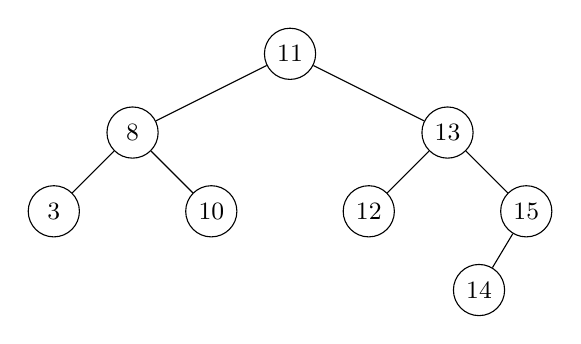
\begin{tikzpicture}[every node/.style={circle,draw,minimum size=6.5mm,inner sep=0pt,font=\small},
  level distance=10mm, level 1/.style={sibling distance=40mm}, level 2/.style={sibling distance=20mm},
  level 3/.style={sibling distance=12mm}]
\node {11}
  child {node {8} child {node {3}} child {node {10}}}
  child {node {13} child {node {12}} child {node {15} child {node {14}} child[missing]}};
\end{tikzpicture}
\end{center}
\begin{itemize}[leftmargin=2.2em]
\item[㈠] 若欲搜尋的鍵值（Key）平均分布在 1 到 100 之間，請算出該值於搜尋樹中平均要比較幾次。（5 分）
\item[㈡] 設鍵值 K＝2 時，其機率為 0.5，K＝5 時其機率為 0.3，K＝9 時其機率為 0.103，其餘 97 個數機率均為
0.001，請算出該值於搜尋樹中要比較幾次。（10 分）
\item[㈢] 設各鍵值的機率如上述第㈡小題，是否能將此搜尋樹重新安排以獲得較佳的平均比較次數？請說明原因或理由。（10 分）
\end{itemize}
\end{pastexam}

\begin{pastsoln}
答案：㈠ 平均 $2.97$ 次；㈡ 期望 $2.997$ 次；㈢ 可以，例如最佳的排法期望只要 $1.79$ 次。

\textbf{計算的約定。} 搜尋從根往下走（資結書虛擬碼~9.1），每經過一個節點就拿 $K$ 和它的鍵比較
一次（一次比較分出「等於、小於、大於」三種結果），等於就成功停下；走到空指標就是搜尋失敗。 所以
比較次數＝路上經過的節點數。 $1$ 到 $100$ 裡只有 $8$ 個數在樹裡，其餘 $92$ 個數的搜尋都是失敗的
搜尋，也要算進去。

\textbf{㈠} 先算每個數要比較幾次。

成功的搜尋（比較次數＝節點的層數，根在第 $1$ 層）：
\begin{center}
\begin{tabular}{lccc}
\toprule
鍵 & 層數 & 個數 & 小計 \\
\midrule
$11$ & 1 & 1 & 1 \\
$8, 13$ & 2 & 2 & 4 \\
$3, 10, 12, 15$ & 3 & 4 & 12 \\
$14$ & 4 & 1 & 4 \\
\midrule
合計 & & 8 & 21 \\
\bottomrule
\end{tabular}
\end{center}

失敗的搜尋：看 $K$ 落在哪兩個相鄰的鍵之間，就知道它掉到哪個空指標。
\begin{itemize}
\item $K = 1, 2$（小於 $3$）：比較 $11, 8, 3$ 後走到 $3$ 的左空指標，$3$ 次。
\item $K = 4 \sim 7$（在 $3$ 和 $8$ 之間）：比較 $11, 8, 3$，走到 $3$ 的右空指標，$3$ 次。
\item $K = 9$（在 $8$ 和 $10$ 之間）：比較 $11, 8, 10$，$3$ 次。
\item $10$ 和 $11$、$11$ 和 $12$、$12$ 和 $13$、$13$ 和 $14$、$14$ 和 $15$ 之間沒有整數。
\item $K = 16 \sim 100$（大於 $15$，共 $85$ 個）：比較 $11, 13, 15$，$3$ 次。
\end{itemize}
失敗的共 $2 + 4 + 1 + 85 = 92$ 個數，每個 $3$ 次，合計 $276$ 次。

全部 $100$ 個數的比較次數總和 $21 + 276 = 297$，每個數機率 $1/100$，平均
\[
\frac{297}{100} = 2.97 \text{ 次}.
\]

\textbf{㈡} $K = 2$、$5$、$9$ 都不在樹裡，由㈠的分析各要比較 $3$ 次。 其餘 $97$ 個數的比較次數總和是
$297 - 3 \times 3 = 288$。 期望比較次數
\[
0.5 \times 3 + 0.3 \times 3 + 0.103 \times 3 + 0.001 \times 288
= 2.709 + 0.288 = 2.997 \text{ 次}.
\]
三個機率加起來 $0.5 + 0.3 + 0.103 + 97 \times 0.001 = 1$，分布合法。

\textbf{㈢ 可以。} 原因：$90.3\%$ 的搜尋是找 $2, 5, 9$，三個都不在樹裡，失敗時停在「小於 $3$」「$3$ 和
$8$ 之間」「$8$ 和 $10$ 之間」這三個空位；這三個空位在原樹裡都在第 $3$ 層的節點下面，每次要比較
$3$ 次。 原樹只照鍵的大小排得平衡，沒有考慮搜尋的機率。 把決定這三個空位的鍵 $3$、$8$、$10$ 移到
靠近根的地方，機率大的搜尋就變短；代價是機率很小的其他搜尋變長，划得來。

把「每個空位被搜尋的機率」也算進權重，用資結書第~18.4~節最佳二元搜尋樹的動態規劃，可以算出
這組機率下最好的排法（同樣這 $8$ 個鍵）。 各空位的機率是：小於 $3$（$K = 1, 2$）$0.501$；$3$ 和
$8$ 之間（$4 \sim 7$）$0.303$；$8$ 和 $10$ 之間（$9$）$0.103$；大於 $15$（$16 \sim 100$）$0.085$；
其他空位 $0$；每個鍵本身 $0.001$。 結果是下面這棵樹：
\begin{center}
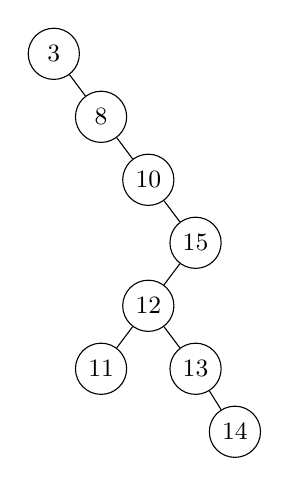
\begin{tikzpicture}[every node/.style={circle,draw,minimum size=6.5mm,inner sep=0pt,font=\small},
  level distance=8mm, level 1/.style={sibling distance=12mm}, level 2/.style={sibling distance=12mm},
  level 3/.style={sibling distance=12mm}, level 4/.style={sibling distance=12mm},
  level 5/.style={sibling distance=12mm}, level 6/.style={sibling distance=10mm}]
\node {3}
  child[missing]
  child {node {8}
    child[missing]
    child {node {10}
      child[missing]
      child {node {15}
        child {node {12} child {node {11}} child {node {13} child[missing] child {node {14}}}}
        child[missing]}}};
\end{tikzpicture}
\end{center}
期望比較次數：
\begin{itemize}
\item $K = 1, 2$：比較 $3$ 就往左掉出去，$1$ 次，貢獻 $0.501 \times 1 = 0.501$。
\item $K = 4 \sim 7$：比較 $3, 8$，$2$ 次，貢獻 $0.303 \times 2 = 0.606$。
\item $K = 9$：比較 $3, 8, 10$，$3$ 次，貢獻 $0.103 \times 3 = 0.309$。
\item $K = 16 \sim 100$：比較 $3, 8, 10, 15$，$4$ 次，貢獻 $0.085 \times 4 = 0.34$。
\item 樹裡的鍵 $3, 8, 10, 15, 12, 11, 13, 14$ 分別在第 $1, 2, 3, 4, 5, 6, 6, 7$ 層，
共 $34$ 次，貢獻 $0.034$。
\end{itemize}
合計 $0.501 + 0.606 + 0.309 + 0.34 + 0.034 = 1.79$ 次，比原樹的 $2.997$ 次少了四成。 這棵樹很
「歪」，但搜尋的機率集中在左邊，歪向機率大的那一邊反而比較好。 不想做動態規劃，只要把 $3$ 放在
根、$8$ 接在 $3$ 的右邊，$K = 2$ 就只要比較 $1$ 次、$K = 5$ 只要 $2$ 次，已經比原樹好很多。
\end{pastsoln}
